%%%%%%%%%%%%%%%%%%%%%%%%%%%%%%%%%%%%%%%%%%%%%%
%Lab report writeup based on template by Derek Hildreth
%%%%%%%%%%%%%%%%%%%%%%%%%%%%%%%%%%%%%%%%%%%%%%

\documentclass[aps,letterpaper,10pt]{article}

\usepackage{graphicx} % For images
\usepackage{float}    % For tables and other floats
\usepackage{verbatim} % For comments and other
\usepackage{amsmath}  % For math
\usepackage{amssymb}  % For more math
\usepackage{fullpage} % Set margins and place page numbers at bottom center
\usepackage{subfig}   % For subfigures
\usepackage[usenames,dvipsnames]{color} % For colors and names
\usepackage{fancyhdr} %headers
\usepackage{wrapfig} % for inline images

\usepackage{easytable}

%%%%%%%%%%%%

%HEADER FORMATING%%%%%%%%%%%%%
\pagestyle{fancy}
\headheight 23pt
\setlength{\headsep}{20pt}
\lhead{18.369 - PSet 2}
\chead{Due 26 Feb 2016}
\rhead{A.G. Athanassiadis}
%%%%%%%%%%%%%%%%%%%%%%%%

%Custom Definitions%%%%%%%%%%%%%%%
\newcommand{\ttt}{\texttt}
\newcommand{\D}[1]{ $D^{(#1)}$ }
%%%%%%%%%%%%%%%%%%%%%%%%

\begin{document}

\begin{figure*}[!h]
\centering
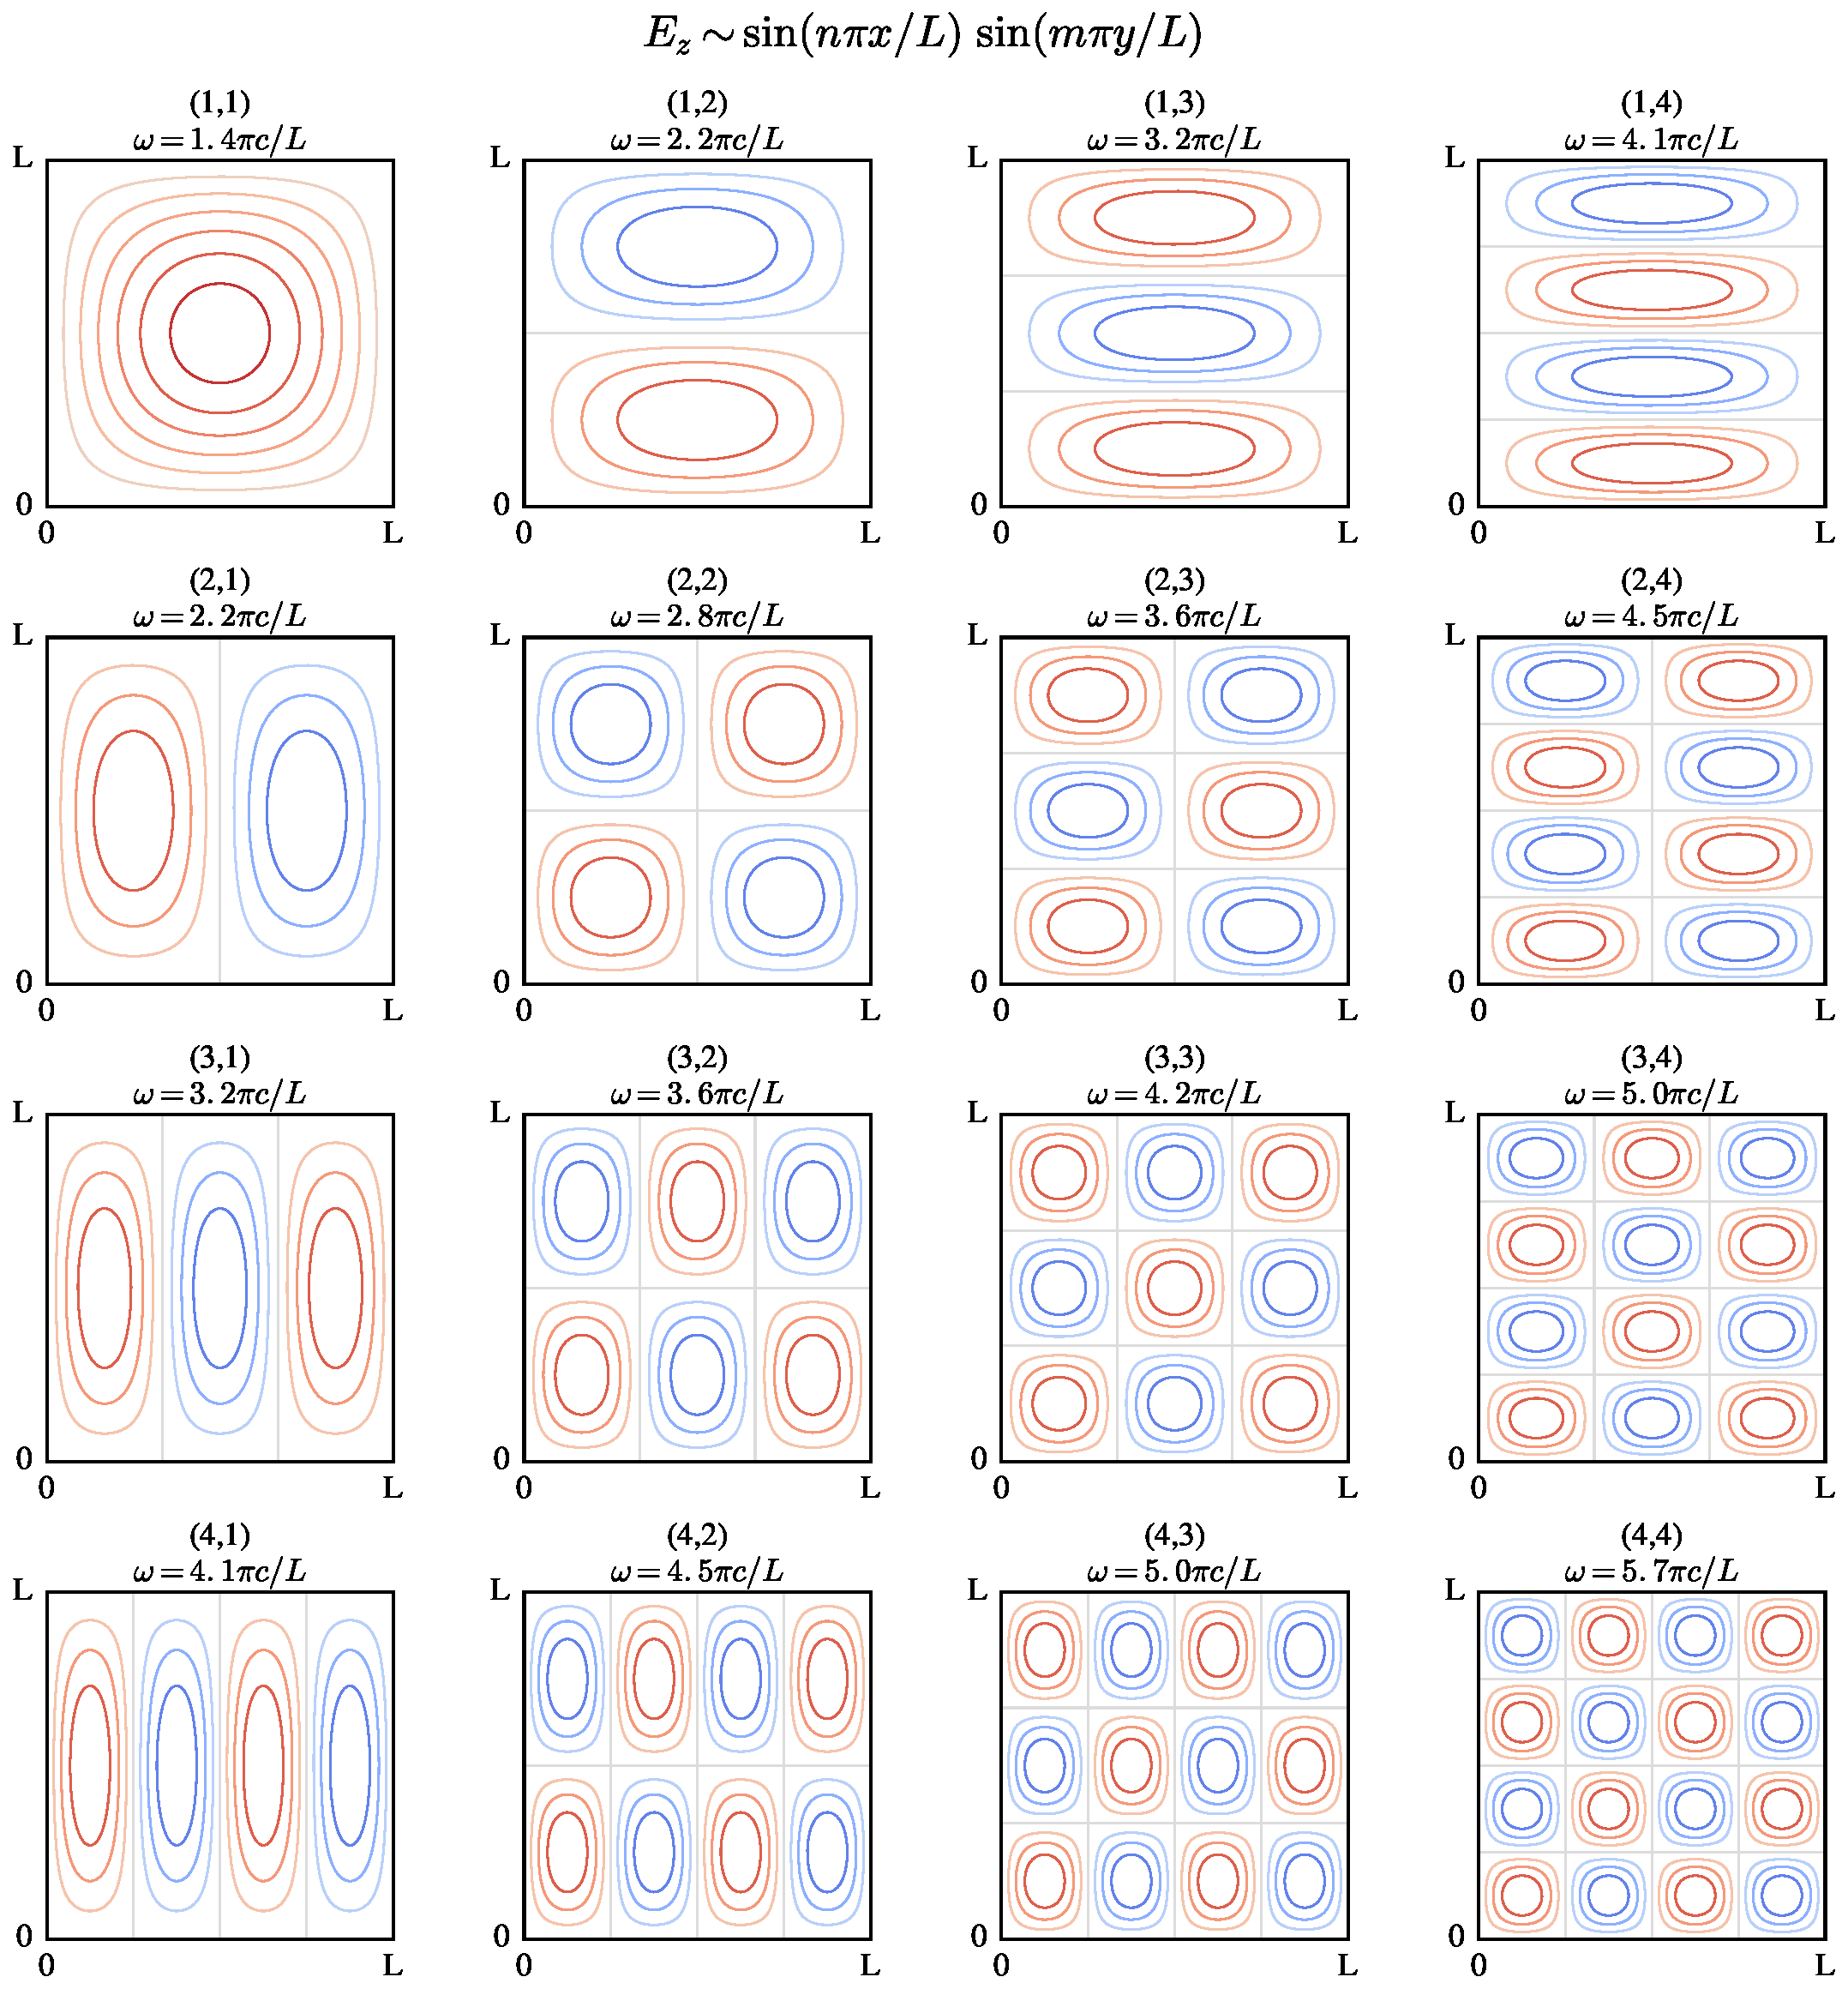
\includegraphics[width=\textwidth]{Soln.pdf}
\caption{\label{fig:all_soln} Eigenfunctions $E_z$ to the problem $\nabla^2 E_z = - \frac{\omega^2}{c^2} E_z,$ organized by the coefficients $(n,m),$ which correspond to the wave number in the $\hat{x}$ and $\hat{y}$ directions respectively. The solution frequencies $\omega$ are provided to illustrate degenerate solutions. Red contours represent positive $E_z$ and blue represent negative $E_z$.}
\end{figure*}

\newpage
\section{Problem 2b}

The solutions for all $(n,m)$ from $(1,1)$ to $(4,4)$ are tabulated in Fig.~\ref{fig:all_soln}. Using these contour plots of the eigenfunctions $(n,m),$ I evaluate which eigenfunctions are partners of the different irreps. 

Note that because the solutions for $E_z \sim \sin(n \pi x / L)\sin(m\pi x/L),$ the solution for $n=0$ or $m=0$ is a trivial solution with zero field everywhere. As such, the $(0,0)$ solution is a partner of irrep \D1 since it transforms identically. Similarly, by inspection, the solution $(1,1)$ is a partner of irrep \D1 since it is even under all transformations. \\

In the following table, the solutions above are organized by their partner irrep. For some of the degenerate eigenfunctions, the nominal solution for $(n,m)$ can be decomposed into the \emph{sum} of two functions that are partners of irreps. These partner functions are represented as $(n,m) \pm (m,n)$ below. Since they are degenerate (with the same $\omega$), these linear combinations of solutions are also valid solutions of the equation \emph{and} are partners of irrep.

\begin{table*}[h!]
\renewcommand{\arraystretch}{2}
\centering
\begin{tabular}{ c|l }
    Irrep &  Partner Functions \\
    \hline
	\D1 & ($n$,0)\quad (0,$m$) \quad(1,1) \quad \{(1,3) + (3,1)\} \quad (3,3) \\
	\D2 & \{(2,4) - (4,2)\} \\
	\D3 & (2,2)\quad \{(1,3)-(3,1)\} \\
	\D4 & \{(2,4) + (4,2)\}\quad (4,4)\\
	\D5 & (1,2)\quad (2,1)\quad (1,4)\quad (4,1)\quad (2,3)\quad (3,2)\quad (3,4)\quad (4,3)\\
\end{tabular}
\end{table*}

The irrep partners were generally found by inspecting the parity under the different transformations. The partners of \D5 are easily identified because they are the only functions that are odd under rotation $C_2.$ Similarly, the partners of \D1 are quick to spot because under all transformations, the solution is retained.\\

The degenerate solutions were sometimes clearly partners of an irrep, and other times needed to be decomposed. The projection operator could be used to find the irrep components, as was done for the degenerate solutions $(2,4)$ and $(4,2)$ below.

\newpage
\subsection{To approaches to decompose degenerate solutions}

\begin{figure*}[!h]
	\centering
	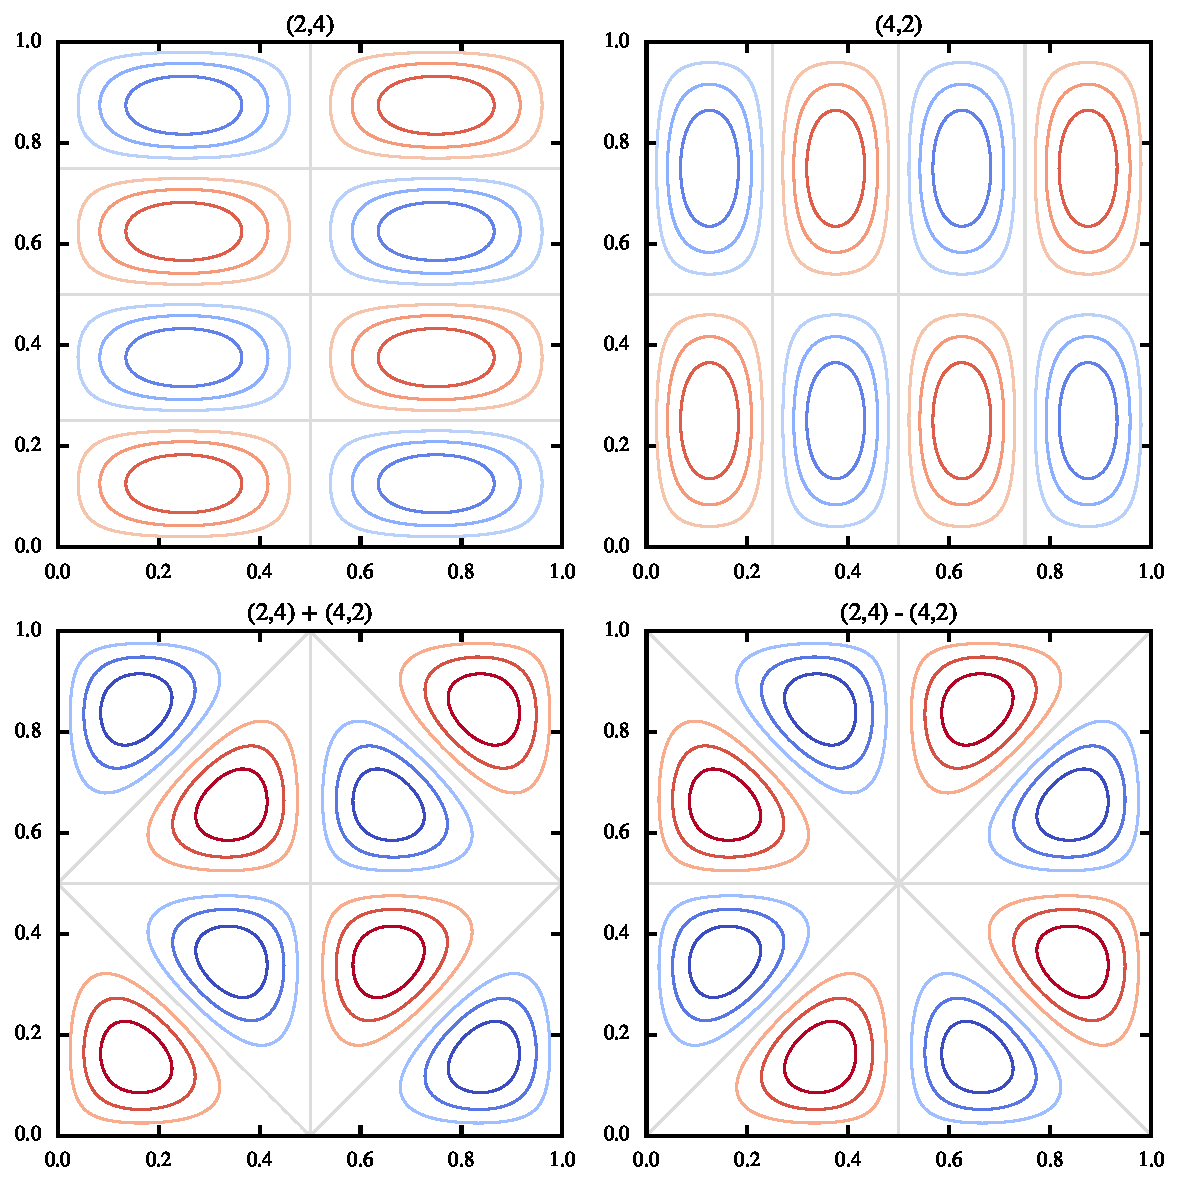
\includegraphics[width=0.6\textwidth]{Soln24-42}
\end{figure*}

By inspection, the solutions (2,4) and (4,2) are not partners of a single irrep, but they can be decomposed.

\{(2,4) + (4,2)\} is even under $\sigma'$, odd under $\sigma$, even under $C_2$ and odd under $C_4$, making it a partner of $D^{(4)}.$ \{(2,4) - (4,2)\} is odd under both $\sigma$ and $\sigma'$ and even under both $C_2$ and $C_2$. Hence this solution is a partner of $D^{(2)}.$ 

Alternately, these partners can be found by projecting either (2,4) or (4,2) onto $D^{(2)}$ and $D^{(4)}:$

\begin{align*}
P^{(2)} E_{24} & = \frac{1}{8} ( E_{24} - \hat{O}_{\sigma_1}E_{24} - \hat{O}_{\sigma_2}E_{24} - \hat{O}_{\sigma_1'}E_{24} - \hat{O}_{\sigma_2'}E_{24} + \hat{O}_{C_4}E_{24} + \hat{O}_{C_4^{-1}}E_{24} + \hat{O}_{C_4}E_{24}) \\
& = \frac{1}{8} (E_{24} - (-E_{24}) - (-E_{24}) - (E_{42}) - (E_{42}) + (-E_{42}) + (-E_{42}) + (E_{24})) \\ 
& = \frac{1}{2} (E_{24} - E_{42})
\end{align*}

\begin{align*}
P^{(4)} E_{24} & = \frac{1}{8} ( E_{24} - \hat{O}_{\sigma_1}E_{24} - \hat{O}_{\sigma_2}E_{24} + \hat{O}_{\sigma_1'}E_{24} + \hat{O}_{\sigma_2'}E_{24} - \hat{O}_{C_4}E_{24} - \hat{O}_{C_4^{-1}}E_{24} + \hat{O}_{C_4}E_{24}) \\
& = \frac{1}{8} (E_{24} - (-E_{24}) - (-E_{24}) + (E_{42}) + (E_{42}) - (-E_{42}) - (-E_{42}) + (E_{24})) \\ 
& = \frac{1}{2} (E_{24} + E_{42})
\end{align*}

Sim for $E_{42}.$

\end{document}